\documentclass[bachelor,zhspacing]{cqu}  %单面打印版本
\usepackage{etex}


%%在这增加你需要的其它包
\definecolor{hellgelb}{rgb}{1,1,0.8}
\definecolor{colKeys}{rgb}{0,0,1}
\definecolor{colIdentifier}{rgb}{0,0,0}
\definecolor{colComments}{rgb}{1,0,0}
\definecolor{colString}{rgb}{0,0.5,0}
\usepackage{listings}
\lstset{%
    float=hbp,%
    basicstyle=\ttfamily\small, %
    identifierstyle=\color{colIdentifier}, %
    keywordstyle=\color{colKeys}, %
    stringstyle=\color{colString}, %
    commentstyle=\color{colComments}, %
    columns=flexible, %
    tabsize=4, %
    frame=single, %
    extendedchars=true, %
    showspaces=false, %
    showstringspaces=false, %
    numbers=left, %
    numberstyle=\tiny, %
    breaklines=true, %
   backgroundcolor=\color{hellgelb}, %
    breakautoindent=true, %
    captionpos=b,%
	xleftmargin=0pt%
}

\begin{document}

%-----------------------------------论文题目-------------------------------------------------
\xuehao{20121892}
\cntitle{重庆大学\LaTeX 学位论文模板CQU使用说明}
\cnauthor{张乐}
\cnmajor{软件工程}
\cnteacher{葛永新}
\cnxueyuan{软件学院}
\entitle{An Instruction of the \LaTeX\ Templet for Chongqing University Thesis}
\enauthor{Le Zhang}
\enmajor{Software Engineering}
\enteacher{Prof. Yongxin Ge}
\enxueyuan{College of Software}
\cnkind{****}
\enkind{****}
%\cnzlteacher{ }  %%助理教师,如果必要,还要将cqu.cls中的有关该项前的%号去掉
%\enzlteacher{ }
\cndate{二O一六年六月}
\endate{June 2016}
%%%%只需修改上面的相关信息%%%%%%%%
\makecntitle 
\makeentitle 
%%%%%%%%%%%%%%%%%%%%%%%%%%%

\pagenumbering{Roman}
\setcounter{page}{0}
%------------------------------------文章摘要------------------------------------------------------------
\cnkeywords{模板,摘要,论文,\LaTeX}
\begin{cnabstract}
摘要是设计或论文内容不加注释和评论的简短陈述,应以第三人称陈述。它应具有独立性和自含性,
即不阅读设计或论文的全文,就能获得必要的信息,摘要的内容应包含与设计或论文同等量的主要信
息,供读者确定有无必要阅读全文,也供文摘等二次文献采用。\par
摘要一般应说明研究工作目的、实验研究方法、结果和最终结论等,而重点是结果和结论。摘要中一
般不用图、表、化学结构式、计算机程序,不用非公知公用的符号、术语和非法定的计量单位。\par
摘要页置于英文题名页后。 \par
中文摘要一般为400汉字左右,用小四号宋体。 \par
关键词是为了文献标引工作从设计(论文)中选取出来用以表示全文主题内容信息款目的单词或术
语。一般每篇设计(论文)应选取3~5个词作为关键词,关键词间用逗号隔开,最后一个词后不打标点
符号。以显著的字符排在同种语言摘要的下方。如有可能,尽量用《汉语主题词表》等词表提供的规
范词。\par
本文介绍重庆大学论文模板cqu的使用方法。本模板符合学校的本科论文格式基本要求,而硕博模板
有待完善。
本文的创新点主要有:
\begin{itemize*}
\item 用例子来解释模板的使用方法;
\item 用废话来填充无关紧要的部分;
\item 一边学习摸索一边编写新代码。
\end{itemize*}
(模板作者注:中文关键词定义cnkeywords应在使用中文摘要环境之前。英文关键词同理。)
\end{cnabstract} 
\enkeywords{template, \LaTeX, abstract, paper}
\begin{enabstract}
     An abstract of a dissertation is a summary and extraction of 
research work and contributions. Included in an abstract should be 
description of research topic and research objective, brief 
introduction to methodology and research process, and summarization 
of conclusion and contributions of the research. An abstract should be 
characterized by independence and clarity and carry identical 
information with the dissertation. It should be such that the general 
idea and major contributions of the dissertation are conveyed
without reading the dissertation.\par
     An abstract should be concise and to the point. It is a 
misunderstanding to make an abstract an outline of the dissertation and 
words “the first chapter”, “the second chapter” and the like should be 
avoided in the abstract.\par
     Key words are terms used in a dissertation for indexing, 
reflecting core information of the dissertation. An abstract may 
contain a maximum of 5 key words, with semicolons used in between to 
separate one another.
\end{enabstract}
%%%%%%%%%%%%%%%%%%%%%%%%%%%%%%%%%%%%%%

%--------------文章目录-------------
\tableofcontents
\listoffigures
%\addcontentsline{toc}{section}{插图清单}
\listoftables
%\addcontentsline{toc}{section}{附表清单}


%------------------------------------词汇------------------------------------------------------------
\begin{denotation}{2.5}{0}

\item[cluster] 集群
\item[Itanium] 安腾
\item[SMP] 对称多处理
\item[API] 应用程序编程接口
\item[PI]   聚酰亚胺
\item[劝  学] 君子曰:学不可以已。青,取之于蓝,而青于蓝;冰,水为之,而寒于水。
  木直中绳。(车柔)以为轮,其曲中规。虽有槁暴,不复挺者,(车柔)使之然也。故木
  受绳则直, 金就砺则利,君子博学而日参省乎己,则知明而行无过矣。吾尝终日而思
  矣,  不如须臾之所学也;吾尝(足齐)而望矣,不如登高之博见也。登高而招,臂非加
  长也,  而见者远;  顺风而呼,  声非加疾也,而闻者彰。假舆马者,非利足也,而致
  千里;假舟楫者,非能水也,而绝江河,  君子生非异也,善假于物也。积土成山,风雨
  兴焉;积水成渊,蛟龙生焉;积善成德,而神明自得,圣心备焉。故不积跬步,无以至千
  里;不积小流,无以成江海。骐骥一跃,不能十步;驽马十驾,功在不舍。锲而舍之,朽
  木不折;  锲而不舍,金石可镂。蚓无爪牙之利,筋骨之强,上食埃土,下饮黄泉,用心
  一也。蟹六跪而二螯,非蛇鳝之穴无可寄托者,用心躁也。\pozhehao{} 荀况
\end{denotation}

%%%%%%%%%%%%%%%%%%%%%%%%%%%%%%%%%%%%%%%

\pagenumbering{arabic}

\section{前言}\label{ux524dux8a00}

当今人们越来越依赖Web服务,如查看E-mail,淘宝购物,百度搜索,这些Web服务已经和我们息息相关,我们很难想象没有他们的生活。而对于这些服务的提供者来说,确保服务资源能真正被用户使用,而不是被恶意机器人使用,是至关重要的。如使用机器人注册账户\textsuperscript{{[}1{]}},不仅会占用宝贵服务器资源,还为发布恶意信息埋下伏笔。所以区分访问来自人类还是机器人是十分重要的,验证码正是因为这个原因而被广泛使用。验证码(CAPTCHA)是``Completely
Automated Public Tests to tell Compu\textsuperscript{{[}2{]}}ters and
Humans
Apart''{[}29,28,27,15,9{]}。的缩写。其主要思想是通过电脑向人类提问,通过回答来区分人和机器人。这个问题需要对人来说简单,而对电脑来说很难(或是需要很长时间)解决。

\section{背景}\label{ux80ccux666f}

目前在互联网上最流行的CAPTCHA系统,是基于文本的。但是,由于计算机视觉技术的提高,基于文本的系统很容易被攻击成功\textsuperscript{{[}3{]}}。所以越来越多的研究者考虑如何替换掉基于文本的系统,于是有基于图像的\textsuperscript{{[}6{]}}和基于声音的\textsuperscript{{[}12{]}}系统。

\subsection{文本验证码系统}\label{ux6587ux672cux9a8cux8bc1ux7801ux7cfbux7edf}

总的来说,基于文本的验证码系统让用户识别字母或数字,GIMPY是一个经典的例子\textsuperscript{{[}2{]}}。攻击基于文本的使用大多使用OCR(optical
character
recognition)。这个技术讲图片分割成晓得区域,每个区域只有一个字母,然后使用模式识别技术使用字母模板匹配每一个区块\textsuperscript{{[}4{]}}。最后一步是一个比较成熟的AI问题。为了防止这样的攻击,基于文本的系统使用如下技术来增强鲁棒性\textsuperscript{{[}14{]}}:

\begin{itemize}
\tightlist
\item
  增加噪音:向图片中增加线和点,来干扰区域分割算法。
\item
  字符扭曲:对字符使用扭曲变换,或3D变换来增加文字识别难度。
\item
  字符连接或重叠:将两个或者多个字母连接或者重叠起来,使得攻击算法无法正确划分图片。
\end{itemize}

\begin{figure}[htbp]
\centering
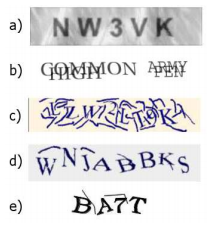
\includegraphics{pic/text-captcha.png}
\caption{一些文本CAPTCHA的例子}\label{pic:text-captcha}
\end{figure}

如@pic:text-captcha,a很容易被OCR破解,b引入了字符的重叠,c引入了噪声,d和e同时引入噪声和字符扭曲。

然而,以上方法在提高系统鲁棒性的同时,也提高了人类识别的难度,特别是字符的连接。如字符``r''和``n''连接起来,看起来就像是字符``m''。字符扭曲也有可能增加用户识别的难度,如扭曲的后的''S``和''5``就很难分辨。还有些系统使用不同的颜色来标示每个字符,而这些都能很容易的被自动化的程序所移除,并没有给机器识别带来任何的难度\textsuperscript{{[}16{]}}。而reCAPTCHA\textsuperscript{{[}17{]}}提供了一种比较好的解决思路:使用两个单词来验证用户,其中一个是确定答案的,另外一个是不确定的。不确定答案的单词来自古籍中无法被自动化OCR程序识别的单词,确定答案的单词是机器生成的或者多个用户的答案是一致的来自古籍中的单词。这个过程既可以起到验证作用又可以数字化图书,是一个非常好的解决方案。但是还是这个解决方案还是有如下缺点:

\begin{itemize}
\tightlist
\item
  对移动用户不友好:移动设备通常屏幕较小,输入困难,输入较长的单词对用户来说是一个极大的负担。
\item
  无法防御基于机器学习的攻击:基于机器学习的攻击,能比较容易的识别文本,此方法对与基于机器学习的攻击没有很好的鲁棒性。
\item
  易导致用户多次刷新:由于一个单词来自古籍,可能出现用户多次刷新来获得清晰可读的验证码,而这对热门Web服务器来说,是一个极大的负担。
\end{itemize}

正是由于基于文本的系统固有的缺点,有了声音验证系统和图像验证码系统。

\subsection{声音验证系统}\label{ux58f0ux97f3ux9a8cux8bc1ux7cfbux7edf}

声音验证码系统弥补来了视觉障碍用户的可用性需求。一般的声音验证码系统让字母和数字被随机的声音间隔隔开,并向其中添加背景噪声。用户只有很少的时间去确定每个单词。某种意义上说,声音验证码系统仅仅是文本验证码系统的听觉版本,用声音替代可视化的东西,并没有明显的增加破解的难度。构成攻击的基础是相似的------特征提取和字符分类。对机器和人的难度曲线是相似的\textsuperscript{{[}18{]}}。所以声音验证码系统既没有提供更加用户友好的接口,也没有更好的防范自动化程序的破解。这也就是它没有被广泛使用的根本原因。

\subsection{图像验证码系统}\label{ux56feux50cfux9a8cux8bc1ux7801ux7cfbux7edf}

图像验证码系统逐渐替代了越来越复杂的文本验证码系统,图像验证码有很好的用户接口,它主要利用人类对图片超乎想象的处理能力来区分人和机器。ESP-PIX\textsuperscript{{[}19{]}}让用户从一系列词中选择能描述素有图片的。SQ-PIX\textsuperscript{{[}20{]}}让用户标示出物品的所在位置,这对图片候选库提出很大要求,大部分图片可能需要人工处理。Google的图片验证码``what's
up''\textsuperscript{{[}7{]}}让用户旋转图片,把图片旋转至正确方向。这个过程需要比较精确的鼠标移动,并且有些图片的方向可能是模棱两可的。Microsoft的Asirra\textsuperscript{{[}6{]}}使用petfinder.com上已有的数据库,让用户在12张图片中找到所有有猫的图片(其他图片都为狗)。而这些图片可能是模棱两可的,如@pic:asirral。这样的验证码这个对于机器来说,难度只有区分狗和猫,而对于人来说,却可能花费很长时间解决。

\begin{figure}[htbp]
\centering
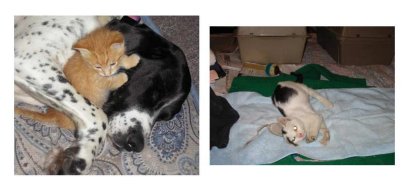
\includegraphics{pic/asirral.png}
\caption{petfinder.com中模棱两可的图片}\label{pic:asirral}
\end{figure}

12306火车购票\textsuperscript{{[}21{]}}让用户从所有图片中选择系统指定内容的图片,如@fig:12306captcha。但是同样也存在一个致命的问题:图片需要人工导入,并手动指定标签。有如下缺点:

\begin{itemize}
\tightlist
\item
  人工失误:人工指定标签时给出错误标签
\item
  易遭受穷举攻击:因为人工指定,图片库不可能太大,穷举所有图片,并自动或手动指定标签即可很好的破解此类验证码
\item
  手工录入的标签信息很难复用:花费大量人力物力输入的信息除了验证码,并不能用在其他地方。
\end{itemize}

\begin{figure}[htbp]
\centering
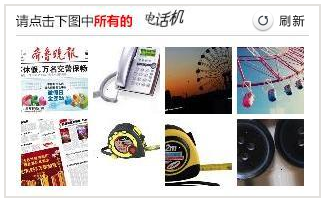
\includegraphics{pic/12306captcha.png}
\caption{12306验证码}\label{fig:12306captcha}
\end{figure}

\hypertarget{refs}{}
\hypertarget{ref-baird2002human}{}
{[}1{]} BAIRD H S, POPAT K. Human interactive proofs and document image
analysis{[}G{]}//Document Analysis Systems V. Springer, 2002: 507--518.

\hypertarget{ref-gimpy}{}
{[}2{]} Gimpy 项目{[}J{]}. \url{http://www.captcha.net/captchas/gimpy/}.

\hypertarget{ref-yan2008low}{}
{[}3{]} YAN J, EL AHMAD A S. A Low-cost Attack on a Microsoft
CAPTCHA{[}C{]}//Proceedings of the 15th ACM conference on Computer and
communications security. ACM, 2008: 543--554.

\hypertarget{ref-mori2003recognizing}{}
{[}4{]} MORI G, MALIK J. Recognizing objects in adversarial clutter:
Breaking a visual CAPTCHA{[}C{]}//Computer Vision and Pattern
Recognition, 2003. Proceedings. 2003 IEEE Computer Society Conference
on. IEEE, 2003, 1: I--134.

\hypertarget{ref-simard2005using}{}
{[}5{]} SIMARD P. Using machine learning to break visual human
interaction proofs (hips{[}J{]}. Advances in neural information
processing systems, 2005, 17: 265--272.

\hypertarget{ref-elson2007asirra}{}
{[}6{]} ELSON J, DOUCEUR J R, HOWELL J, 等. Asirra: a CAPTCHA that
exploits interest-aligned manual image categorization.{[}C{]}//2007.

\hypertarget{ref-gossweiler2009s}{}
{[}7{]} GOSSWEILER R, KAMVAR M, BALUJA S. What's up CAPTCHA?: a CAPTCHA
based on image orientation{[}C{]}//Proceedings of the 18th international
conference on World wide web. ACM, 2009: 841--850.

\hypertarget{ref-chew2004image}{}
{[}8{]} CHEW M, TYGAR J D. Image recognition captchas{[}M{]}. Springer,
2004.

\hypertarget{ref-datta2005imagination}{}
{[}9{]} DATTA R, LI J, WANG J Z. IMAGINATION: a robust image-based
CAPTCHA generation system{[}C{]}//Proceedings of the 13th annual ACM
international conference on Multimedia. ACM, 2005: 331--334.

\hypertarget{ref-matthews2010scene}{}
{[}10{]} MATTHEWS P, MANTEL A, ZOU C C. Scene tagging: image-based
CAPTCHA using image composition and object
relationships{[}C{]}//Proceedings of the 5th ACM Symposium on
Information, Computer and Communications Security. ACM, 2010: 345--350.

\hypertarget{ref-zhu2010attacks}{}
{[}11{]} ZHU B B, YAN J, LI Q, 等. Attacks and design of image
recognition CAPTCHAs{[}C{]}//Proceedings of the 17th ACM conference on
Computer and communications security. ACM, 2010: 187--200.

\hypertarget{ref-chan2003using}{}
{[}12{]} CHAN T-Y. Using a test-to-speech synthesizer to generate a
reverse Turing test{[}C{]}//Tools with Artificial Intelligence, 2003.
Proceedings. 15th IEEE International Conference on. IEEE, 2003:
226--232.

\hypertarget{ref-bigham2009evaluating}{}
{[}13{]} BIGHAM J P, CAVENDER A C. Evaluating existing audio CAPTCHAs
and an interface optimized for non-visual use{[}C{]}//Proceedings of the
SIGCHI Conference on Human Factors in Computing Systems. ACM, 2009:
1829--1838.

\hypertarget{ref-el2010robustness}{}
{[}14{]} EL AHMAD A S, YAN J, MARSHALL L. The robustness of a new
CAPTCHA{[}C{]}//Proceedings of the Third European Workshop on System
Security. ACM, 2010: 36--41.

\hypertarget{ref-chellapilla2005designing}{}
{[}15{]} CHELLAPILLA K, LARSON K, SIMARD P, 等. Designing human friendly
human interaction proofs (HIPs){[}C{]}//Proceedings of the SIGCHI
conference on Human factors in computing systems. ACM, 2005: 711--720.

\hypertarget{ref-yan2008usability}{}
{[}16{]} YAN J, EL AHMAD A S. Usability of CAPTCHAs or usability issues
in CAPTCHA design{[}C{]}//Proceedings of the 4th symposium on Usable
privacy and security. ACM, 2008: 44--52.

\hypertarget{ref-googlerecaptcha}{}
{[}17{]} Google reCAPTCHA 项目{[}J{]}.
\url{https://www.google.com/recaptcha/intro/index.html}.

\hypertarget{ref-bursztein2011failure}{}
{[}18{]} BURSZTEIN E, BEAUXIS R, PASKOV H, 等. The failure of
noise-based non-continuous audio captchas{[}C{]}//Security and Privacy
(SP), 2011 IEEE Symposium on. IEEE, 2011: 19--31.

\hypertarget{ref-esp-pix}{}
{[}19{]} Esp-pix{[}J{]}.
\url{http://server251.theory.cs.cmu.edu/cgi-bin/esp-pix/esp-pix}.

\hypertarget{ref-sq-pix}{}
{[}20{]} Sq-pix{[}J{]}.
\url{http://server251.theory.cs.cmu.edu/cgi-bin/sq-pix}.

\hypertarget{ref-captcha12306}{}
{[}21{]} 12306验证码{[}J{]}. \url{https://kyfw.12306.cn/otn/login/init}.

%\include{chapters/summery}

%%%%%%%%%%%%%%%%%%%%%%%%%%%%%%%%%%%%%%%



%\include{chapters/appendix}  %%附录

\end{document}
